\documentclass[comsoc, journal]{IEEEtran}
\usepackage{blindtext}
\usepackage{graphicx}
\usepackage{url}
\usepackage[spanish]{babel}
\selectlanguage{spanish}
\usepackage[utf8]{inputenc}
\usepackage{listings}

\hyphenation{op-tical net-works semi-conduc-tor}


\begin{document}
\title{Primer trabajo teoría de la información y la comunicación}
\author{Miguel~Angel~Asencio~Hurtado, Ana~María~Rodríguez~Reyes% <-this % stops a space
}

\markboth{Teoría de la información y la comunicación - Universidad Nacional de Colombia}%
{Shell \MakeLowercase{\textit{et al.}}: Bare Demo of IEEEtran.cls for Journals}

\maketitle


\begin{abstract}
Se plantean diferentes problemas y sus respectivas soluciones en los temas de tratamiento de señales, aliasing, transformada de Fourier y señales de audio
\end{abstract}

\begin{IEEEkeywords}
audio, Fourier, MATLAB, frecuencia, señales, aliasing
\end{IEEEkeywords}

\IEEEpeerreviewmaketitle

\section{Objetivos}

\begin{itemize}
    \item Entender el funcionamiento de MATLAB, como grabar sonido, reproducir sonido y generar interfaces gráficas
    \item Ver ejemplos de como se genera el Aliasing
    \item Probar diferentes métodos de interpolación
    \item Poder escuchar los colores (sinusoides con las mismas frecuencias)
\end{itemize}

\section{Marco teórico}
\subsection{Señal periodica}
\subsubsection{Definición}
Una función es periódica si verifica la condición $f(x + T) = f(x)$; el número  $T$  se llama período de la función. Generalmente, se llama período al menor número real positivo $T$ que satiface la condición. Las funciones trigonométricas son ejemplos sencillos de una función periódica, que en combinaciones adecuadas se emplean en el análisis armónico \cite{encyc}.

\subsubsection{Frecuencia}
Frecuencia es una magnitud que mide el número de repeticiones por unidad de tiempo de cualquier fenómeno o suceso periódico. Para calcular la frecuencia de un suceso, se contabilizan un número de ocurrencias de este teniendo en cuenta un intervalo temporal, luego estas repeticiones se dividen por el tiempo transcurrido. Según el Sistema Internacional (SI), la frecuencia se mide en hercios (Hz), en honor a Heinrich Rudolf Hertz. Un hercio es la frecuencia de un suceso o fenómeno repetido una vez por segundo.

Un método alternativo para calcular la frecuencia es medir el tiempo entre dos repeticiones (periodo) y luego calcular la frecuencia (f) recíproca de esta manera:

$$f = \frac{1}{T}$$

donde T es el periodo de la señal \cite{serway}.
\subsubsection{Periodo}
Es el mínimo lapso que separa dos instantes en los que el sistema se encuentra exactamente en el mismo estado: mismas posiciones, mismas velocidades, mismas amplitudes. Así, el periodo de oscilación de una onda es el tiempo empleado por la misma en completar una longitud de onda. En términos breves es el tiempo que dura un ciclo de la onda en volver a comenzar. Por ejemplo, en una onda, el periodo es el tiempo transcurrido entre dos crestas o valles sucesivos \cite{serway}:

$$T = \frac {2\pi}{\omega}$$

\subsection{Convertidor análogo digital}
Un conversor o convertidor de señal analógica a digital (Conversor Analógico Digital, CAD; Analog-to-Digital Converter, ADC) es un dispositivo electrónico capaz de convertir una señal analógica, ya sea de tensión o corriente, en una señal digital mediante un cuantificador y codificándose en muchos casos en un código binario en particular. Donde un código es la representación unívoca de los elementos, en este caso, cada valor numérico binario hace corresponder a un solo valor de tensión o corriente.

La digitalización o conversión A/D, básicamente, consiste en realizar de forma periódica medidas de la amplitud (tensión) de una señal; por ejemplo, la que proviene de un micrófono \cite{walden}.

\subsection{Interpolación}
En el subcampo matemático del análisis numérico, se denomina interpolación a la obtención de nuevos puntos partiendo del conocimiento de un conjunto discreto de puntos o la aproximación de una función de calculo costoso por una más sencilla \cite{crochiere}.

\subsection{Aliasing}
Es el efecto que causa que señales continuas distintas se tornen indistinguibles cuando se muestrean digitalmente. Cuando esto sucede, la señal original no puede ser reconstruida de forma unívoca a partir de la señal digital. Una imagen limitada en banda y muestreada por debajo de su frecuencia de Nyquist en las direcciones ``x'' e ``y'', resulta en una superposición de las replicaciones periódicas del espectro $G(f_x, f_y)$. Este fenómeno de superposición periódica sucesiva es lo que se conoce como aliasing o Efecto Nyquist.

El aliasing es un motivo de preocupación mayor en lo que concierne a la conversión analógica-digital de señales de audio y vídeo: el muestreo incorrecto de señales analógicas puede provocar que señales de alta frecuencia presenten dicho aliasing con respecto a señales de baja frecuencia. El aliasing es también una preocupación en el área de la computación gráfica e infografía, donde puede dar origen a patrones de moiré (en las imágenes con muchos detalles finos) y también a bordes dentados \cite{serway}.

\subsection{Teorema del muestreo}
El teorema de muestreo de Nyquist-Shannon, también conocido como teorema de muestreo de Whittaker-Nyquist-Kotelnikov-Shannon, teorema de Nyquist o teorema del muestreo, es un teorema fundamental de la teoría de la información, de especial interés en las telecomunicaciones. Este teorema fue formulado en forma de conjetura por primera vez por Harry Nyquist en 1928 (Certain topics in telegraph transmission theory), y fue demostrado formalmente por Claude E. Shannon en 1949 (Communication in the presence of noise).

El teorema demuestra que la reconstrucción exacta de una señal periódica continua en banda base a partir de sus muestras, es matemáticamente posible si la señal está limitada en banda y la tasa de muestreo es superior al doble de su ancho de banda.

Dicho de otro modo, la información completa de la señal analógica original que cumple el criterio anterior está descrita por la serie total de muestras que resultaron del proceso de muestreo. No hay nada, por tanto, de la evolución de la señal entre muestras que no esté perfectamente definido por la serie total de muestras.

Si la frecuencia más alta contenida en una señal analógica $x_a(t)$, es $F_{max}=B$, y la señal se muestrea a una tasa $F_s>2F_{max} \equiv 2B$, entonces $x_a(t)$, se puede recuperar totalmente a partir de sus muestras mediante la siguiente función de interpolación:

$$g(t) = \frac{\sin 2 \pi B t}{2 \pi B t}$$

Así, $x_a(t)$ , se puede expresar como:

$$x_a(t) = \sum_{n=-\infty}^{\infty} x_a \left(\frac{n}{F_s}\right) g \left(t-\frac{n}{F_s}\right)$$

donde $x_a \left(\frac{n}{F_s}\right)= x_a \left(nT\right) \equiv x \left(n\right)$ son las muestras de $x_a \left(t\right)$ \cite{nyquist}.

\subsection{Serie de Fourier}
Una serie de Fourier es una serie infinita que converge puntualmente a una función periódica y continua a trozos (o por partes). Las series de Fourier constituyen la herramienta matemática básica del análisis de Fourier empleado para analizar funciones periódicas a través de la descomposición de dicha función en una suma infinita de funciones sinusoidales mucho más simples (como combinación de senos y cosenos con frecuencias enteras). El nombre se debe al matemático francés Jean-Baptiste Joseph Fourier, que desarrolló la teoría cuando estudiaba la ecuación del calor. Fue el primero que estudió tales series sistemáticamente, y publicó sus resultados iniciales en 1807 y 1811. Esta área de investigación se llama algunas veces análisis armónico.

Las series de Fourier tienen la forma:

$$\frac{a_0}{2} + \sum_{n=1}^\infty\left[a_n\cos\frac{2n\pi}{T}t + b_n\sin\frac{2n\pi}{T}t\right]$$

Donde $a_n$, y $b_n$, se denominan coeficientes de Fourier de la serie de Fourier de la función $f(x)$ \cite{spiegel}.

\subsection{Transformada de Fourier}
La transformada de Fourier, denominada así por Joseph Fourier, es una transformación matemática empleada para transformar señales entre el dominio del tiempo (o espacial) y el dominio de la frecuencia, que tiene muchas aplicaciones en la física y la ingeniería. Es reversible, siendo capaz de transformaciones de cualquiera de los dominios al otro. El propio término se refiere tanto a la operación de transformación como a la función que produce.

La transformada de Fourier es una aplicación que hace corresponder a una función $f$ de valores complejos y definida en la recta, con otra función $g$ definida de la manera siguiente:

$$g(\xi ) =  \frac{1}{\sqrt{2\pi}}\int_{-\infty}^{+\infty} f(x)e^{-i\xi\,x} dx$$

En la práctica las variables $x$ y $\xi$ suelen estar asociadas a dimensiones como el tiempo y frecuencia \cite{spiegel}.

\section{Desarrollo}
\subsection{Aliasing}
Se desea ver el fenómeno de aliasing entre dos señales, de manera que en una señal de frecuencia de $1Hz$ con un muestreo de frecuencia menor a $2f$, genere una señal de frecuencia $\frac{1}{4}Hz$.

Para lograr esto se realizan varios experimentos, midiendo con frecuencia de 1 (Figura~\ref{fig_al_1}), 1.25 (Figura~\ref{fig_al_125}), 1.125 (Figura~\ref{fig_al_25}), 4 (Figura~\ref{fig_al_4}) y 8 (Figura~\ref{fig_al_8}).

\begin{figure}[!t]
\centering
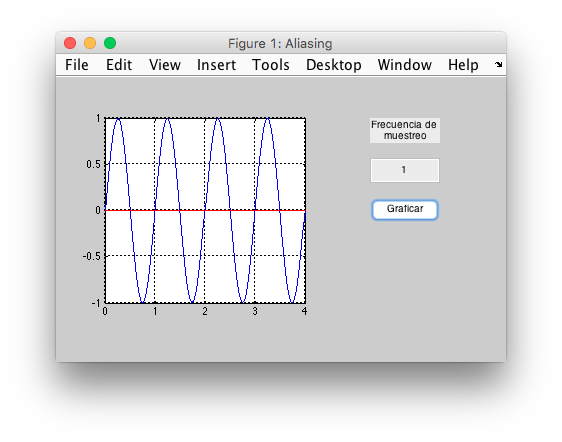
\includegraphics[width=3.5in]{imgs/aliasing_1.png}
\caption{Frecuencia de muestreo de 1}
\label{fig_al_1}
\end{figure}

\begin{figure}[!t]
\centering
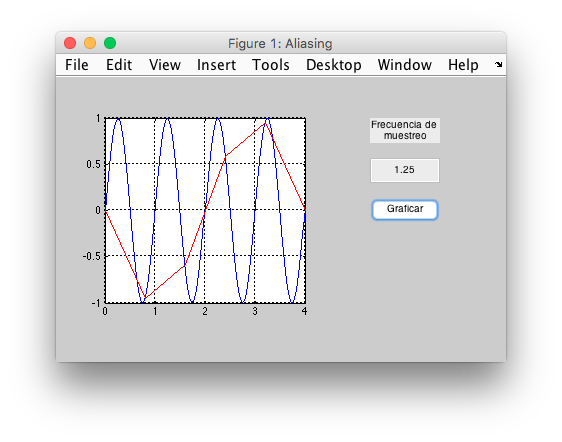
\includegraphics[width=3.5in]{imgs/aliasing_25.png}
\caption{Frecuencia de muestreo de 1.25}
\label{fig_al_25}
\end{figure}

\begin{figure}[!t]
\centering
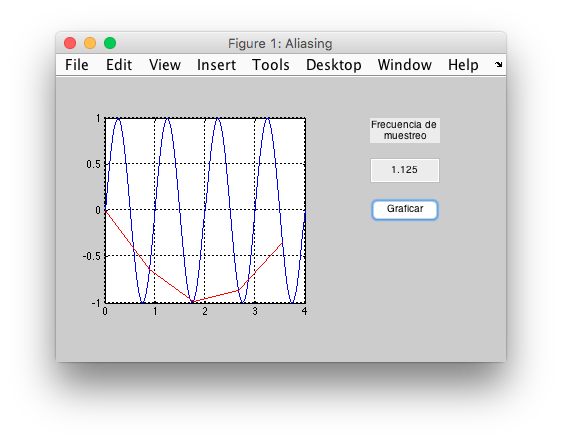
\includegraphics[width=3.5in]{imgs/aliasing_125.png}
\caption{Frecuencia de muestreo de 1.125}
\label{fig_al_125}
\end{figure}

\begin{figure}[!t]
\centering
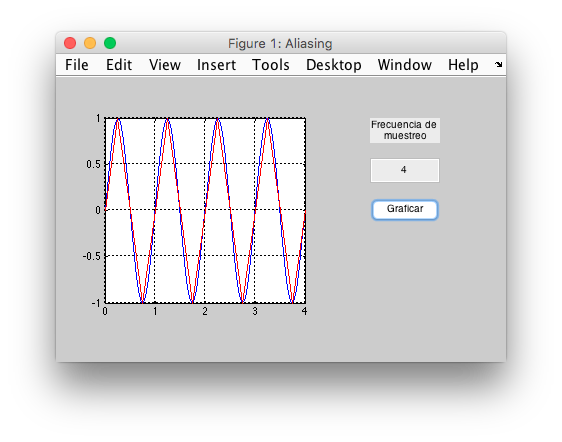
\includegraphics[width=3.5in]{imgs/aliasing_4.png}
\caption{Frecuencia de muestreo de 4}
\label{fig_al_4}
\end{figure}

\begin{figure}[!t]
\centering
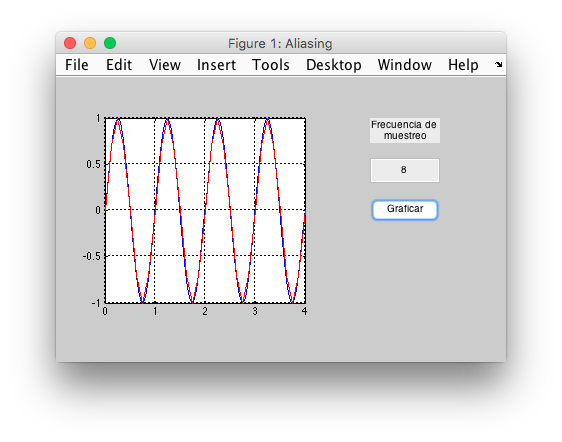
\includegraphics[width=3.5in]{imgs/aliasing_8.png}
\caption{Frecuencia de muestreo de 8}
\label{fig_al_8}
\end{figure}

\subsection{Voz}
En esta sección se realizan diferentes experimentos sobre la voz para poder observar aspectos como: su representación en frecuencia y en tiempo. La interfaz gráfica desarrollada para este fin se puede observar en la figura \ref{voz_1} . 

\subsubsection{Grabar voz}

Para grabar la voz se utiliza recordblocking a la cual se le asigna un audiorecorder como se muestra en el Código \ref{matlab_voice} , en el cual se pueden establecer los parámetros de grabación como: frecuencia, canal (mono o estéreo) y bits. La grabación se realiza por 5 segundos.

\begin{lstlisting}[caption={Grabar voz},label={matlab_voice},language=Matlab]
recObj = audiorecorder;
recordblocking(recObj, 5);
\end{lstlisting}

\subsubsection{Reproducir voz}

Para reproducir la voz grabada, primero se debe obtener una la información del  audio con la función  getaudiodata(), y luego esta se pasa como argumento a sound() que es la encargada de reproducir los sonidos junto con la frecuencia a la que se quiere reproducir el audio, en este caso este valor se define en la interfaz gráfica. 

\begin{lstlisting}[caption={Reproducir sonido},label={matlab_playsound},language=Matlab]
	y = getaudiodata(recObj);    
    sound(y, Fs);
\end{lstlisting}

\subsubsection{Reproducción inversa de la voz}

Teniendo la grabación de la voz, se desea reproducir la misma de manera inversa, para este caso se utiliza la función flipud(), que se encarga de invertir el arreglo numérico que representa la voz.

\subsubsection{Representación en tiempo y en frecuencia}

Buscando tener una representación en frecuencia de la voz grabada, se debe aplicar primero la transformada de Fourier a la misma lo que se puede hacer en Matlab con la función fft como se ve el Código \ref{matlab_fft}, con ella obtenemos los componentes de frecuencia y a partir de se obtiene la gráfica. Esto se realiza para la grabación de voz normal y la invertida.

\begin{lstlisting}[caption={Representación en frecuencia},label={matlab_fft},language=Matlab]
	y3 = fft(y);
	L = 5000;
	P2 = abs(y3/L);
	P1 = P2(1:L/2+1);
	P1(2:end-1) = 2*P1(2:end-1);
	d_fs = Fs*(0:(L/2))/L;
	plot(d_fs, P1)
\end{lstlisting}

\begin{figure}[!t]
\centering
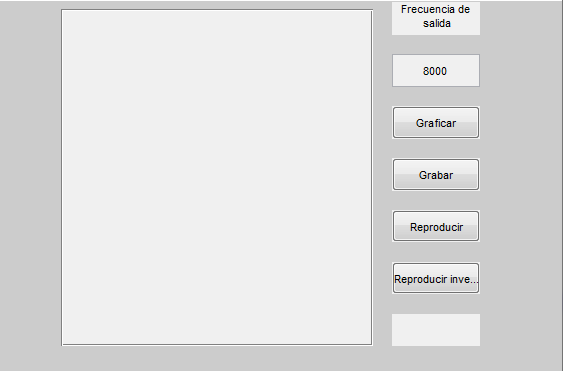
\includegraphics[width=3.5in]{imgs/voz_1.png}
\caption{Interfaz gráfica para experimentos de voz}
\label{voz_1}
\end{figure}

\begin{figure}[!t]
\centering
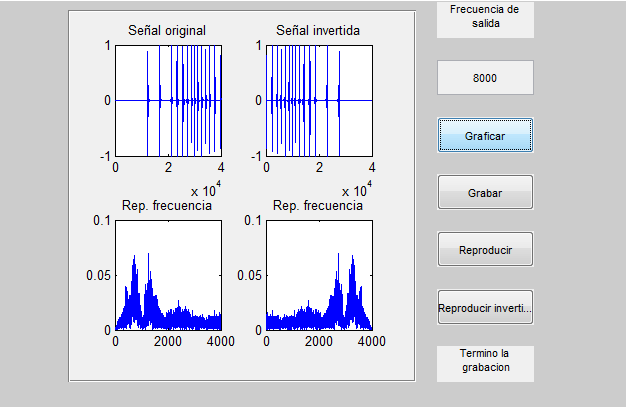
\includegraphics[width=3.5in]{imgs/voz_2.png}
\caption{Interfaz gráfica para experimentos de voz}
\label{voz_2}
\end{figure}

\subsection{Escuchar colores}
Se desea ser capaz de escuchar los colores. Para esto se construye una sinusoide con una frecuencia igual a la del color que se desea escuchar. Los colores con su respectiva frecuencia se pueden ver en el Cuadro~\ref{table_color} \cite{bohren}.

\begin{table}[!t]
    \renewcommand{\arraystretch}{1.3}
    \caption{Rango de frecuencia de los colores}
    \label{table_color}
    \centering
    \begin{tabular}{|c|c|}
        \hline
        Color & Frecuencia (THz)\\
        \hline
        Red	    & 430 - 480\\
        \hline
        Orange	& 480 - 510\\
        \hline
        Yellow	& 510 - 540\\
        \hline
        Green	& 540 - 580\\
        \hline
        Cyan	& 580 - 610\\
        \hline
        Blue	& 610 - 670\\
        \hline
        Violet	& 670 - 750\\
        \hline
    \end{tabular}
\end{table}

Dado que el espectro audible del humano se encuentra entre 20Hz y 20kHz \cite{rosen}, las frecuencias exeden la capacidad auditiva, por lo que a manera académica se toman en vez de THz como Hz y de esta manera ya se encuentran el rango audible.

\subsection{Interpolación}
TODO

\section{Análisis de resultados}
\subsection{Aliasing}
Como se esperaba se ve que en las frecuencias mayores a la frecuencia de Nyquist (Figuras \ref{fig_al_4} y \ref{fig_al_8}) la señal se asemeja a la señal original, mientras que para las frecuencias menores (Figuras \ref{fig_al_1}, \ref{fig_al_25} y \ref{fig_al_125}) la señal resultante difiere de la señal original, presentandose el fenómeno de aliasing.

Tambien es visible que para el caso de la señal con frecuencia de muestreo de 1.25 (Figura~\ref{fig_al_25}), la frecuencia resultante para la señal generada es de 0.25Hz, situación que se repite con la señal con frecuencia de muestreo de 1.125 (Figura~\ref{fig_al_125}), la cual tiene una frecuencia resultante de 0.125Hz.

\subsection{Grabar voz}
Al aumentar la frecuencia de muestreo en la grabación de voz se puede escuchar la grabación más grave y lenta, mientras que al disminuirla de escucha la grabación más aguda y rápida. Este efecto también se presenta al cambiar la frecuencia de muestreo en la reproducción, pero se presenta de manera contraria, ya que al aumentar la frecuencia se escucha la grabación más aguda y al disminuirla se escucha más grave.

\subsection{Escuchar colores}
Las frecuencias de los colores, como se encuentran fuera del rango audible, al generar una señal senoidal con esta frecuencia es imposible poder escucharla, pero al realizar el cambio unidades de THz a Hz, se pueden ya escuchar las diferentes tonalidades de colores.

\subsection{Interpolación}
TODO

\section{Conclusiones}
\begin{itemize}
    \item Toda señal tiene un contenido frecuencial que puede ser observado por medio de la transformada de Fourier.
    \item Los dispositivos de computo, al ser elementos discretos, obligan a usar el teorema del muestreo, ya que al no usarse, puede presentarse el aliasing y con esto no solo hay perdida de información si no que pueden haber datos erroneos.
    \item Al cambiar la frecuencia de muestreo en grabación de voz se genera un fenómeno de aliasing, sonando más grave o más aguda.
    \item Aunque los colores también son señales, el contenido de frecuencia de estas señales se encuentran fuera de la capacidad auditiva del ser humano.
\end{itemize}

\ifCLASSOPTIONcaptionsoff
  \newpage
\fi

\begin{thebibliography}{1}

\bibitem{encyc}
Encyclopedia of math: periodic function,
\url{https://goo.gl/416jzE}

\bibitem{serway}
Serway, Raymond A.; Jewett, John W. (2004). Physics for Scientists and Engineers (6ª edición). Brooks/Cole.

\bibitem{walden}
Walden, R. H. (1999). Analog-to-digital converter survey and analysis. IEEE Journal on Selected Areas in Communications

\bibitem{crochiere}
R.E. Crochiere and L.R. Rabiner. (1983). Multirate Digital Signal Processing. Englewood Cliffs, NJ: Prentice–Hall.

\bibitem{nyquist}
H. Nyquist, Certain topics in telegraph transmission theory, Trans. AIEE, volumen 47, páginas 617-644, abril de 1928.

\bibitem{spiegel}
M. R. Spiegel, J. Liu, L. Abellanas (2003): Fórmulas y tablas de matemática aplicada. Segunda edición. Serie Schaum. Mc Graw-Hill.

\bibitem{bohren}
Craig F. Bohren (2006). Fundamentals of Atmospheric Radiation: An Introduction with 400 Problems. Wiley-VCH. ISBN 3-527-40503-8.

\bibitem{rosen}
Rosen, Stuart (2011). Signals and Systems for Speech and Hearing (2nd ed.). BRILL. p. 163. For auditory signals and human listeners, the accepted range is 20Hz to 20kHz, the limits of human hearing

\end{thebibliography}
\end{document}
